\documentclass[titlepage]{article}

\usepackage{amsfonts} 
\usepackage{amsmath}
\usepackage[margin=2.5cm]{geometry}
\usepackage{enumitem}
\usepackage{amsthm}
\usepackage{multirow}
\usepackage{listings}
\usepackage{xcolor}
\usepackage{graphicx}
\usepackage{hyperref}
\usepackage{subcaption}
\usepackage{tocloft}
\usepackage[german]{babel}
\usepackage{mathtools}

\renewcommand\thesection{Aufgabe~\arabic{section}:}
\renewcommand\thesubsection{Teilaufgabe~\arabic{section}\alph{subsection}}
% \renewcommand\theappendix{asdf}

\renewcommand\cftsecnumwidth{7em}
\renewcommand\cftsubsecnumwidth{8em}

\renewcommand*{\proofname}{Beweis}
\newenvironment{ausarbeitung}{\vspace{3mm}\noindent\textit{Ausarbeitung.}}{}

\definecolor{codegreen}{rgb}{0,0.6,0}
\definecolor{codegray}{rgb}{0.5,0.5,0.5}
\definecolor{codepurple}{rgb}{0.58,0,0.82}
\definecolor{backcolour}{rgb}{0.95,0.95,0.92}

\lstdefinestyle{mystyle}{
	backgroundcolor=\color{backcolour},   
	commentstyle=\color{codegreen},
	keywordstyle=\color{magenta},
	numberstyle=\tiny\color{codegray},
	stringstyle=\color{codepurple},
	basicstyle=\ttfamily\footnotesize,
	breakatwhitespace=false,         
	breaklines=true,                 
	captionpos=b,                    
	keepspaces=true,                 
	numbers=left,                    
	numbersep=5pt,                  
	showspaces=false,                
	showstringspaces=false,
	showtabs=false,                  
	tabsize=2
}

\lstset{style=mystyle}


%opening
\title{Abschlussprojekt Numerische Mathematik:\\
	Cholesky-Zerlegung von Skyline-Matrizen}
\author{Ida Hönigmann \and Fabian Dopf}

\begin{document}

\maketitle

\tableofcontents
\newpage


\section{Aufwandsordnung numerischer Verfahren}
Wir betrachten ein abstraktes numerisches Verfahren, das für $N \in \mathbb{N}$ Eingabedaten eine Laufzeit von $y_N \in \mathbb{R}_+$ hat. Man sagt, das Verfahren habe Aufwandsordnung $p > 0$, falls eine Konstante $C > 0$ existiert, sodass $y_N \leq C N^p$ für alle $N \in \mathbb{N}$.

\subsection{}
Die Aufwandsordnung lässt sich über die Folge $\{p_N\}_{N \in \mathbb{N}}$ mit

\begin{align}
	\label{eq:def_N}
	p_N = \frac{\log(y_{2N})-\log(y_n)}{\log(2)} \text{ für } N \in \mathbb{N}
\end{align}

quantifizieren. Beachten Sie, dass die Bestimmung von $p_N$ die Verfügbarkeit von zwei aufeinanderfolgenden Folgengliedern $y_N$ und $y_{2N}$ erfordert. Verwenden Sie den Ansatz $y_N = CN^p$ und leiten Sie die Formel in \ref{eq:def_N} her!

\begin{proof}
	Sei $(y_N)_{N \in \mathbb{N}}$ die Laufzeit eines numerischen Verfahrens. Wir verwenden den Ansatz $y_N = C N^p$ für ein $C>0$ und $N \in \mathbb{N}$.

	Durch Umformen ergibt sich

	\begin{align*}
		&\log(y_{2N}) - \log(y_N) = \log\left(\frac{y_{2N}}{y_N}\right) = \log\left(\frac{C(2N)^{p}}{C\cdot N^{p}}\right) = \log(2^{p}) = p \log(2) \text{ , d.h.} \\
		&p = \frac{\log(y_{2N}) - \log(y_N)}{\log(2)}.
	\end{align*}

	Verhält sich also $y_N$ asymptotisch wie $CN^p$, so konvergiert $p_N$ gegen $p$.

\end{proof}


\subsection{}
Sei $\{\delta_N\}_{N \in \mathbb{N}} \subseteq \mathbb{R}$ eine Nullfolge, d.h. es gilt $\delta_N \rightarrow 0$ für $N \rightarrow \infty$. Weiters verhalte sich die Laufzeit wie $y_N = (C+\delta_N)N^p$ mit $C > 0$. Zeigen Sie, dass die Folge $\{p_N\}_{N \in \mathbb{N}}$ gegen $p$ konvergiert, d.h. es gilt $p_N \rightarrow p$ für $N \rightarrow \infty$.

\begin{proof}	
	Zuerst berechnen wir einen Grenzwert, den wir in späterer Folge verwenden werden.
	
	% \stackrel{\eqref{...}}{=} woher kommen die zwei unterscheidlichen labels??
	
	\begin{align*}
		\lim\limits_{n\rightarrow\infty} \log\left(\frac{C+\delta_{2N}}{C+\delta_N}\right) \stackrel{(1)}{=} \log\left(\lim\limits_{n\rightarrow\infty}\frac{C+\delta_{2N}}{C+\delta_N}\right) = \log\left(\frac{\lim\limits_{n\rightarrow\infty}C+\delta_{2N}}{\lim\limits_{n\rightarrow\infty}C+\delta_N}\right) \stackrel{(2)}{=} \log\left(\frac{C}{C}\right) = \log(1) = 0
	\end{align*}

	Hierbei folgt (1) aus der Stetigkeit des Logarithmus und (2) aus der Voraussetzung $\delta_N\rightarrow 0$ (womit auch $\delta_{2N}\rightarrow 0$).
	
	Setzen wir nun die Voraussetzung $y_N = (C+\delta_N)N^p$ in Gleichung \ref{eq:def_N} ein, so erhalten wir

	\begin{align*}
		p_N &= \frac{\log(y_{2N}) - \log(y_N)}{\log(2)} = \frac{\log((C+\delta_{2N})(2N)^p) - \log((C+\delta_N)N^p)}{\log(2)} = \frac{\log\left(\frac{(C+\delta_{2N})(2N)^p}{(C+\delta_N)N^p}\right)}{\log(2)} \\
		&= \frac{\log\left(\frac{(C+\delta_{2N})2^p}{(C+\delta_N)}\right)}{\log(2)} = \frac{p \log(2) + \log\left(\frac{C+\delta_{2N}}{C+\delta_N}\right)}{\log(2)} = p + \frac{\log\left(\frac{C+\delta_{2N}}{C+\delta_N}\right)}{\log(2)} \xrightarrow{n\rightarrow\infty} p + 0 = p
	\end{align*}
	
	Zusammenfassend gilt nun $\lim\limits_{n\rightarrow\infty}p_n = p$, was zu zeigen war.

\end{proof}


\subsection{}
In sogenannter doppelt logarithmischer Darstellung (log-log Plots) wird für beide Koordinatenachsen eine logarithmische Skalierung verwendet, d.h. sowohl die waagrechte als auch die senkrechte Koordinatenachse wird logarithmisch unterteilt. Wie werden Potenzfunktionen der Form $y = c x^p$ in einem log-log Plot dargestellt? Wie können Sie die Ordnung $p$ und die Konstante $c > 0$ aus einem log-log Plot von $y = cx^p$ direkt auslesen?

\begin{ausarbeitung}
	Berechnen wir für eine Funktion der Form $y=cx^p$ die Werte $X=\log x$ und $Y = \log y$, so erhalten wir
	
	\begin{align}
		Y = \log y = \log(c x^p) = \log c + p \log x = \log c + p X
	\end{align}

	was der Gleichung einer Geraden entspricht.

	Um den Wert von $c$ abzulesen, kann man den Funktionswert bei $1$ ablesen, da $f(1) = c \cdot 1^p = c$. Um $p$ abzulesen, kann man die Steigung der Geraden ansehen, wenn beide Achsen ''gleich'' skaliert, da $p$ die Steigung der Geraden in Gleichung \ref{eq:log_log} ist.
	
	\begin{figure}
		\centering
		\begin{subfigure}{0.48\textwidth}
			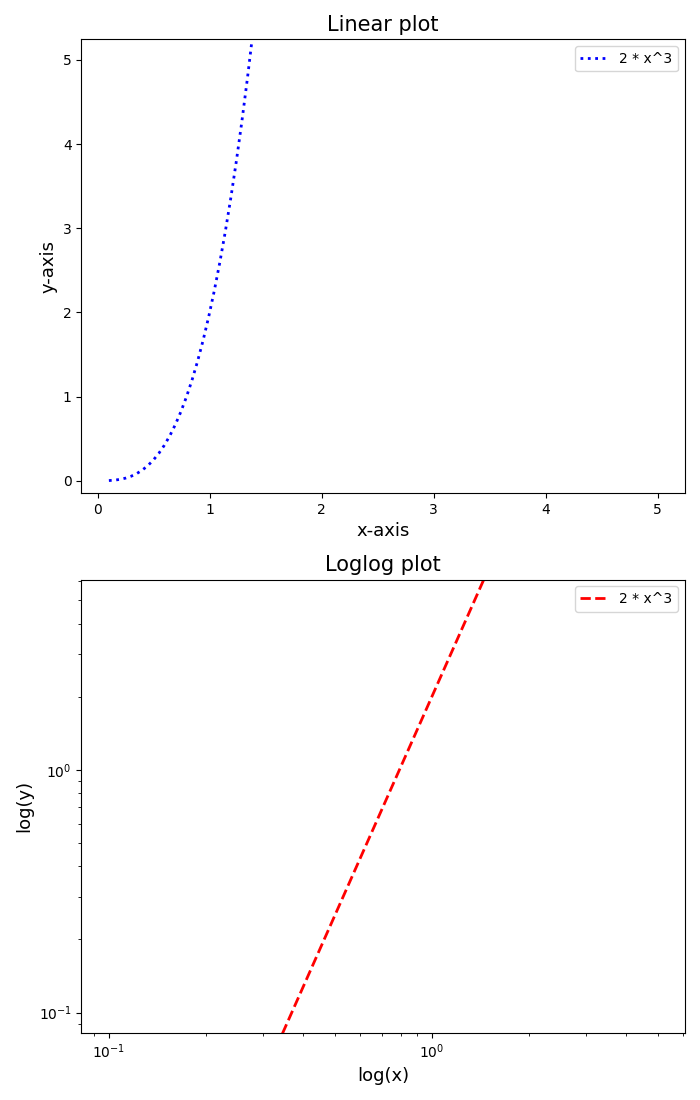
\includegraphics[width=\textwidth]{loglog_plot_a}
			\caption{Vergleich der beiden Graphen der Gleichung $y = 2x^3$. Im Loglog plot ist zu erkennen, dass die Steigung der Geraden $3$ bei gleichen Achsenskalierungen ist, also gilt $p = 3$.}
			\label{fig:loglog_plot_a}
		\end{subfigure}
		\hfill
		\begin{subfigure}{0.48\textwidth}
			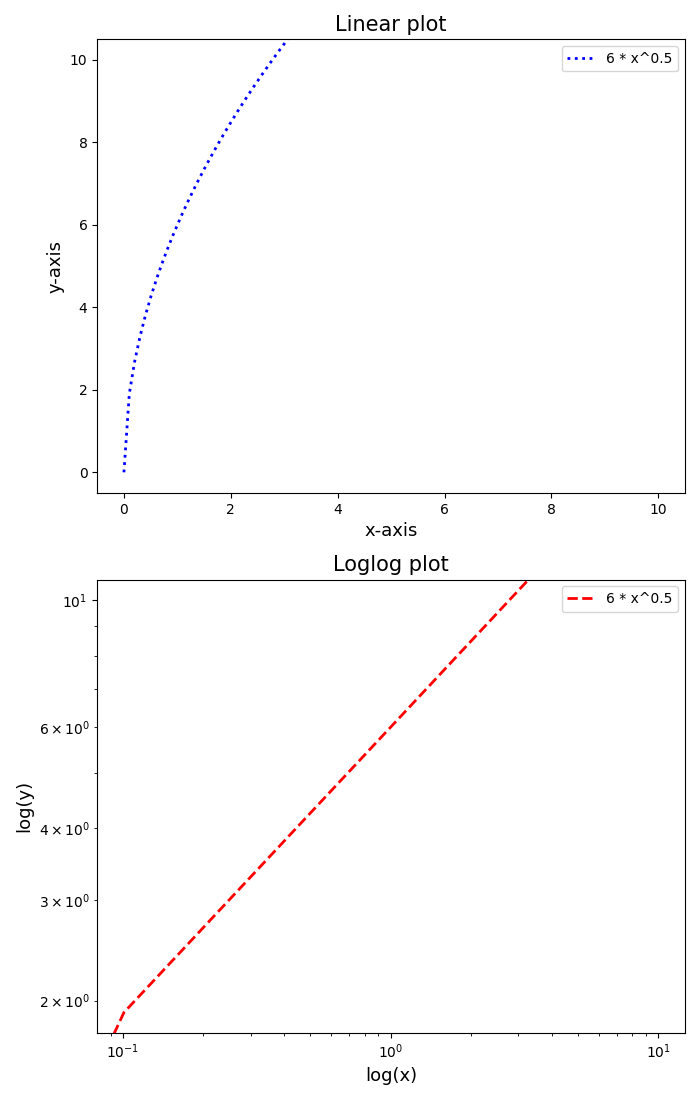
\includegraphics[width=\textwidth]{loglog_plot_b}
			\caption{Vergleich der beiden Graphen der Gleichung $y = 6x^{0.5}$. Im Loglog plot ist zu erkennen, dass bei die Funktion bei $x=1$ den Funktionswert $6$ annimmt, also gilt $c = 6$.}
			\label{fig:loglog_plot_b}
		\end{subfigure}
		
		\caption{Zwei unterschiedliche Funktionen der Form $y = cx^p$, jeweils in einem linear skalierten und einem Loglog Plot.}
		\label{fig:loglog_plot}
	\end{figure}
	
\end{ausarbeitung}
\newpage



\section{Cholesky-Verfahren und Skyline-Matrizen}
Eine Matrix $A \in \mathbb{R}^{n\times n}$ heißt Skyline-Matrix, falls es für $l = 1, ..., n$ Zahlen $p_l, q_l \in \mathbb{N}_0$ gibt, sodass für die $i$-te Zeile und $j$-te Spalte von $A$ gilt:

\begin{itemize}
	\item $A_{i,k} = 0 \text{ für } k < i - p_i$,
	\item $A_{k,j} = 0 \text{ für } k < j - q_j$,
\end{itemize}

Folgendes Beispiel illustriert diese Aussage:

\begin{align*}
	A = \begin{pmatrix}
		1 &   &   &   & 1 \\
		  & 1 &   & 2 & 2 \\
		  &   & 1 & 3 & 3 \\
		1 & 2 & 3 &14 &18 \\
		  & 4 & 5 &29 &48 \\
	\end{pmatrix}.
\end{align*}


\subsection{}
Beweisen Sie, dass das Cholesky-Verfahren genau dann wohldefiniert ist (d.h. es wird nicht durch Null dividiert oder die Wurzel aus einer negativen Zahl gezogen), wenn die Matrix $A \in \mathbb{R}^{n\times n}$ symmetrisch und positiv definit ist.

\begin{proof}
	Wir wiederholen zuerst die relevanten Definitionen.
	
	\begin{itemize}
		\item Eine Matrix $A \in \mathbb{R}^{n\times n}$ heißt symmetrisch, falls $A = A^T$.
		\item Eine Matrix $A \in \mathbb{R}^{n\times n}$ heißt positiv definit, falls $\forall u \in \mathbb{R}^n\setminus\{0\}: u^T A u > 0$.
	\end{itemize}

	Wir zeigen, dass für jede SPD Matrix $A \in \mathbb{R}^{n\times n}$ eine untere Dreiecksmatrix $L \in \mathbb{R}^{n\times n}$ existiert, sodass $LL^T=A$, durch vollständige Induktion nach $n$:
	
	\begin{itemize}
		\item \textbf{Induktionsanfang:} $n=1$
		
		Wenn $A := \begin{pmatrix}
			a_{11}
		\end{pmatrix} \in \mathbb{R}^{1\times 1}$ eine beliebige SPD Matrix ist, so folgt für $u := \begin{pmatrix} 1 \end{pmatrix} \in \mathbb{R}^1 \setminus\{0\}$
		\begin{align*}
			0 < u^TAu = \begin{pmatrix}
				1
			\end{pmatrix} \begin{pmatrix}
				a_{11}
			\end{pmatrix} \begin{pmatrix}
				1
			\end{pmatrix} = a_{11}.
		\end{align*}
	
		Da also $a_{11} > 0$ gilt, ist $L := \begin{pmatrix}
			\sqrt{a_{11}}
		\end{pmatrix} \in \mathbb{R}^{1}$ wohldefiniert. Dann gilt
	
		\begin{align*}
			LL^T = \begin{pmatrix}
				\sqrt{a_{11}}
			\end{pmatrix} \begin{pmatrix}
				\sqrt{a_{11}}
			\end{pmatrix} = \begin{pmatrix}
				a_{11}
			\end{pmatrix} = A.
		\end{align*}
	
		\item \textbf{Induktionsvoraussetzung:} $\forall A \in \mathbb{R}^{n - 1 \times n - 1}$ SPD $\exists L \in \mathbb{R}^{n - 1\times n - 1}$ untere Dreiecksmatrix $:LL^T=A$.
		
		\item \textbf{Induktionsschritt:} $n-1 \implies n$
		
		Sei $A \in \mathbb{R}^{n\times n}$ eine symmetrische und positiv definite Matrix. Wir definieren eine Matrix $B \in \mathbb{R}^{(n-1)\times(n-1)}$, einen Vektor $a \in \mathbb{R}^{n-1}$ und eine Zahl $\alpha \in \mathbb{R}$ durch
		
		\begin{align*}
			\forall i, j \in \{1, ..., n - 1\}: B_{i,j} := A_{i,j}, && \forall i \in \{1, ..., n - 1\}: a_i := A_{i,n}, && \alpha := A_{n,n}.
		\end{align*}
		
		Zusammengefasst gilt nun wegen der Symmetrie von $A$
		
		\begin{align*}
			A = \begin{pmatrix}
				B & a \\
				a^T & \alpha
			\end{pmatrix}
		\end{align*}
	
		$B$ ist eine symmetrische, positiv definite Matrix aus $\mathbb{R}^{(n-1)\times(n-1)}$, daher existiert laut Induktionsvoraussetzung eine untere Dreiecksmatrix $P \in \mathbb{R}^{(n-1)\times(n-1)}$ mit $PP^T=B$.
		
		Da $B$ positiv definit ist und somit regulär ist, folgt die eindeutige Existenz eines Vektors $l \in \mathbb{R}^{n-1}$ der die Gleichung $Pl=a$ erfüllt.
		
		Wir wollen nun $\beta \in \mathbb{R}$ so definieren, dass $\beta = \sqrt{\alpha - l^Tl}$. Dazu müssen wir sicherstellen, dass $\alpha - l^Tl > 0$.
		
		Wenn wir die Definition von $l$ verwenden und Umformen erhalten wir
		
		\begin{align*}
			\alpha - l^Tl &= \alpha - (P^{-1}a)^T(P^{-1}a) = \alpha - a^T (P^{-1})^TP^{-1}a \\
			&= \alpha - a^T (PP^T)^{-1}a = \alpha - a^T B^{-1}a.
		\end{align*}
	
		Da $A$ positiv definit ist ergibt sich
	
		\begin{align*}
			0 < \begin{pmatrix}
				-B^{-1}a\\
				1
			\end{pmatrix}^T
			\underbrace{\begin{pmatrix}
				B & a\\
				a^T & \alpha
			\end{pmatrix}}_{=A}
			\begin{pmatrix}
				-B^{-1}a\\
				1
			\end{pmatrix} =
			\alpha - a^T B^{-1} a.
		\end{align*}
	
		Also ist $\beta := \sqrt{\alpha - l^Tl}$ wohldefiniert. Umgeformt gilt nun $l^Tl + \beta^2 = \alpha$.
		
		Definieren wir nun $L \in \mathbb{R}^{n\times n}$ durch
		
		\begin{align*}
			L = \begin{pmatrix}
				P & 0 \\
				l^T & \beta
			\end{pmatrix},
		\end{align*}
	
		Dann gilt
		
		\begin{align*}
			LL^T = \begin{pmatrix}
				P & 0 \\
				l^T & \beta
			\end{pmatrix} \begin{pmatrix}
				P^T & l \\
				0 & \beta
			\end{pmatrix} = \begin{pmatrix}
				PP^T & Pl \\
				l^TP^T & l^Tl+\beta^2
			\end{pmatrix} = \begin{pmatrix}
				PP^T & Pl \\
				(Pl)^T & l^Tl+\beta^2
			\end{pmatrix} = \begin{pmatrix}
				B & a \\
				a^T & \alpha
			\end{pmatrix} = A,
		\end{align*}
	
		was zu zeigen war.
	\end{itemize}
	
\end{proof}


\subsection{}
Beweisen Sie, dass die Besetzungsstruktur der Cholesky-Zerlegung der Skyline-Matrix $A$ erhalten bleibt, d.h. dass auch die untere Dreiecksmatrix $L$ eine geeignete Bandstruktur aufweist.

\begin{proof}
	Aus der Vorlesung ist bekannt, dass der folgende Algorithmus die Choleksy-Zerlegung einer symmetrischen, positiv definiten Matrix berechnet.
	\begin{enumerate}[label={(\arabic*)}]
		\item \texttt{for k = 1:n}
		\item \hspace{5mm} $L_{kk} = \sqrt{A_{kk} - \sum_{j=1}^{k-1}(L_{kj})^2}$
		\item \hspace{5mm} \texttt{for i = k+1:n}
		\item \hspace{10mm} $L_{ik} = (A_{ik} - \sum_{j=1}^{k-1}L_{ij}L_{kj})/(L_{kk})$
		\item \hspace{5mm} \texttt{end loop}
		\item \texttt{end loop}
	\end{enumerate}

	Weiters ist bekannt, dass im Algorithmus auf Werte $L_{ik}$ nur zugegriffen wird, falls diese bereits berechnet wurden.
	
	Sei $A \in \mathbb{R}^{n\times n}$ eine beliebige symmetrische, positiv definite Skyline Matrix mit $p_l = q_l \in \{1, ..., l\}$, d.h.
	\begin{align*}
		A_{ik} = 0 \text{ für } i,k \in \{1, ..., n\} \text{ mit } k < i - p_i.
	\end{align*}
	
	Sei $L \in \mathbb{R}^{n\times n}$ die untere Dreiecksmatrix aus der Cholesky-Zerlegung. Sei $i \in \{1, ..., n\}$ beliebig.
	
	Wir zeigen
	\begin{align}
		\forall k \in \{1, ..., i - p_i - 1\}: L_{ik} = 0
	\end{align}
	durch vollständige Induktion nach $k$:
	
	Falls $\{1, ..., i - p_i - 1\} = \emptyset$ ist nichts zu zeigen.
	
	\begin{enumerate}
		\item \textbf{Induktionsanfang:} $k=1$
		
		Für $k=1$ gilt
		\begin{align*}
			1 \leq i - p_i - 1 \iff 1 < i - p_i \implies A_{i1} = 0.
		\end{align*}
		
		$L_{i1}$ wird in Zeile 4 des Algorithmus wie folgt berechnet und danach nicht mehr geändert:
		\begin{align*}
			L_{i1} = \frac{A_{i1} - \sum_{j=1}^{0}L_{ij}L_{1j}}{L_{11}} = \frac{0}{L_{11}} = 0
		\end{align*}
	
		\item \textbf{Induktionsvoraussetzung:} Es gelte $\forall j \in \{1, ..., k - 1\}: L_{ij} = 0$.
		
		\item \textbf{Induktionsschritt:} $k-1 \implies k$
		
		Für $k$ gilt
		\begin{align*}
			k \leq i - p_i - 1 \iff k < i - p_i \implies A_{ik} = 0.
		\end{align*}
		
		$L_{ik}$ wird in Zeile 4 des Algorithmus wie folgt berechnet und danach nicht mehr geändert:
		\begin{align*}
			L_{ik} = \frac{A_{ik} - \sum_{j=1}^{k-1}L_{ij}L_{kj}}{L_{kk}} = \frac{0 - \sum_{j=1}^{k - 1}0\cdot L_{kj}}{L_{kk}} = 0
		\end{align*}
	\end{enumerate}
	
	Dadurch ist gezeigt, dass die Skyline-Form in der unteren Dreieckshälfte der Cholesky-Zerlegung erhalten bleibt.
\end{proof}
\newpage



\section{Pseudocode für Cholesky-Zerlegung von Skyline-Matrizen}
Verwenden Sie den Cholesky-Algorithmus aus der Vorlesung. Entwerfen Sie jeweils einen Pseudocode, der für eine Skyline-Matrix:


\subsection{}
möglichst effizient die Struktur erkennt.

\begin{ausarbeitung}
	\begin{lstlisting}[language=Python, caption=Strukturerkennung einer nicht notwendigerweise symmetrischen Skyline-Matrix]
	def to_skyline(matrix):
		values = list()
	
		for i in range(dim(matrix)):
			up_branch = matrix[:, i][:i + 1]	# i-th column from top to diagonal
			up_branch.reverse()
 	    
			# remove all entries outside of skyline-branch
			while not up_branch.empty and up_branch[-1] == 0: 
				up_branch.pop(-1)
	
			left_branch = matrix[i, :][:i]		# i-th row from left to diagonal
			left_branch.reverse()
			
			# remove all entries outside of skyline-branch
			while not left_branch.empty and left_branch[-1] == 0:
				left_branch.pop(-1)
			
			values.append([up_branch, left_branch])
	
		return values
	\end{lstlisting}
	
	\begin{lstlisting}[language=Python, caption=Strukturerkennung einer symmetrischen positiv definiten Skyline-Matrix]
	def to_spd_skyline(matrix):
		values = list()
			
		for i in range(dim(matrix)):
			branch = matrix[:, i][:i + 1]	# i-th column (= row) from top to diagonal
			branch.reverse()
		
			# remove all entries outside of skyline-branch
			while not branch.empty and branch[-1] == 0:
				branch.pop(-1)
				
			values.append(branch)
			
		return values
	\end{lstlisting}
\end{ausarbeitung}


\subsection{}
die Cholesky-Zerlegung berechnet.

\begin{ausarbeitung}
	\begin{lstlisting}[language=Python, caption=Algorithmus für die Cholesky Zerlegung einer Matrix aus der Vorlesung]
	def cholesky(matrix):	
		n = dim(matrix)
		l = zero matrix of dimension n by n

		for k in range(n):
			s = 0
			for j in range(k):
				s += l[k, j] * l[k, j]

			l[k, k] = sqrt(matrix[k, k] - s)

			for i in range(k+1, n):
				s = 0
				for j in range(k):
					s += l[i, j] * l[k, j]

				l[i, k] = (matrix[i, k] - s) / l[k, k]

		return l
	\end{lstlisting}
	
	\begin{lstlisting}[language=Python, caption=Optimierter Algorithmus für die Cholesky Zerlegung einer Skyline-Matrix]
	def cholesky_skyline(values):	# input should be generated by to_spd_skyline
		n = len(values)
		l = zero matrix of dimension n by n

		# calculate maximum branch length
		max_width = max(len(branch) for branch in values)

		for k in range(n):
			# calculate index of first entry not equal to zero
			start_idx = k - len(values[k]) + 1
			# realize sum as dot product of two vectors
			s = np.dot(l[k][start_idx:k], l[k][start_idx:k])
			l[k, k] = sqrt(self[k, k] - s)

			for i in range(k + 1, min(k + max_width, n)):
				if k > i - len(values[i]):	# values outside of the branch are zero
					# realize sum as dot product of two vectors
					s = np.dot(l[i][start_idx:k], l[k][start_idx:k])
					l[i, k] = (self[i, k] - s) / l[k, k]

		return l
	\end{lstlisting}
\end{ausarbeitung}
\newpage



\section{Aufwand des Algorithmus und Verhalten in Spezialfällen}


\subsection{}
Sei $A \in \mathbb{R}^{n\times n}$ eine Skyline-Matrix. Welchen Aufwand haben Ihre Algorithmen aus Aufgabe 3 in Abhängigkeit von der Größe $n$ der Eingabedaten und Skyline-Indices $p_l = q_l$?

\begin{ausarbeitung}
	
	\begin{itemize}
		\item \texttt{to\_skyline} hat wegen den Schleifen in Zeile 4, 9 und 16 Aufwand
		\begin{align*}
			\sum_{l=1}^{n} (n-p_l)+(n-q_l) = 2n^2-\sum_{l=1}^{n}p_l+q_l.
		\end{align*}
		
		\begin{itemize}
			\item best case: Im besten Fall ist $p_l = q_l = l$ also maximal, mit Aufwand
			\begin{align*}
				2n^2-\sum_{l=1}^{n}2l = 2n^2 - 2\frac{n(n+1)}{2} = 2n^2-(n^2+n) = n^2 - n
			\end{align*}
			
			\item worst case: Im schlechtesten Fall ist $p_l = q_l = 0$ also minimal, mit Aufwand
			\begin{align*}
				2n^2 - \sum_{l=1}^{n}0 = 2n^2
			\end{align*}
		\end{itemize}
		
		\item \texttt{to\_spd\_skyline} hat wegen den Schleifen in Zeile 4 und 9 Aufwand 
		\begin{align*}
			\sum_{l=1}^{n}(n-p_l) = n^2 - \sum_{l=1}^{n}p_l
		\end{align*}
		\begin{itemize}
			\item best case: Im besten Fall ist $p_l = l$ also maximal, mit Aufwand 
			\begin{align*}
				n^2 - \sum_{l=1}^{n}l = n^2 - \frac{n(n+1)}{2} = n^2 - \frac{1}{2}n^2 - \frac{1}{2}n = \frac{1}{2}(n^2-n)
			\end{align*}
			\item worst case: Im schlechtesten Fall ist $p_l=1$ also minimal, mit Aufwand 
			\begin{align*}
				n^2 - \sum_{l=1}^{n}1 = n^2 - n
			\end{align*}
		\end{itemize}
	
		\item \texttt{cholesky} hat wegen den Schleifen in Zeile 5, 7, 12 und 14 Aufwand
		\begin{align*}
			\sum_{k=1}^{n}(k + \sum_{i=k+1}^{n}k) &= \sum_{k=1}^{n}(k+k(n-k)) = \sum_{k=1}^{n}k + \sum_{k=1}^{n}kn - \sum_{k=1}^{n}k^2 \\
			&= \frac{n(n+1)}{2} + \frac{n^2(n+1)}{2} - \frac{n(n+1)(2n+1)}{6} = \frac{1}{6}n^3 + \frac{1}{2}n^2 + \frac{1}{3}n
		\end{align*}
		
		also $\mathcal{O}(n^3)$.
		
		\item \texttt{cholesky\_skyline} Zeilen 12 und 18 haben Aufwand $\mathcal{O}(p_k)$, da die beiden Vektoren Länge
		\begin{align*}
			k - start\_idx + 1 = k - (k - p_k + 1) + 1 = p_k
		\end{align*}
		haben und sind somit, neben Zeile 6 mit Aufwand von $\mathcal{O}(n)$, die aufwändigsten Zeilen in der Funktion.
		
		Durch das if-Statement in Zeile 16 wird sichergestellt, dass der Aufwand nur anfällt, falls nach Aufgabe 2b das Ergebnis nicht trivial ist.
		
		Die Einschränkung in Zeile 15 auf den Bereich \texttt{range(k+1, k+max\_width)} statt \texttt{range(k+1, n)} ermöglicht es viele der if-Statements zu ersparen, die es dem Python-Interpreter erschweren die Ausführung zu optimieren\footnote{If-Statements ermöglichen es nicht die Instruction Pipeline vollständig auszunützen und verlangsamen dadurch die Ausführung. In modernen Systemen wird daher sogenannte Branch Prediction durchgeführt die versucht vorherzusagen ob die Bedingung wahr ist.}.
		
		Insgesamt ist der Aufwand also
		\begin{align*}
			n + \sum_{k=1}^{n} \sum_{l=1}^{p_k}p_k = n + \sum_{k=1}^{n} p_k^2
		\end{align*}
		was
		\begin{itemize}
			\item im besten Fall $n + \sum_{k=1}^{n} 1 = 2n = \mathcal{O}(n)$,
			\item im Fall, dass $p_l \approx \sqrt{n}$ ungefähr $n + \sum_{k=1}^{n}(\sqrt{n})^2 = n + n^2 = \mathcal{O}(n^2)$ und
			\item im schlechtesten Fall $n + \sum_{k=1}^{n}k^2 = n + \frac{n(n+1)(2n+1)}{6} = \frac{1}{3}n^3 + \frac{1}{2}n^2 + \frac{7}{6}n = \mathcal{O}(n^3)$ ist.
		\end{itemize}
	\end{itemize}
	
\end{ausarbeitung}


\subsection{}
Betrachten Sie Matrizen mit den Besetzungsstrukturen

\begin{align*}
	\begin{pmatrix}
		* & * & * & * & *\\
		* & * &   &   &  \\
		* &   & * &   &  \\
		* &   &   & * &  \\
		* &   &   &   & *\\
	\end{pmatrix}
	\text{ bzw. }
	\begin{pmatrix}
	* &   &   &   & *\\
	  & * &   &   & *\\
	  &   & * &   & *\\
	  &   &   & * & *\\
	* & * & * & * & *\\
\end{pmatrix}
\end{align*}

Welche Besetzungsstruktur hat die Cholesky-Zerlegung für beide Matrizen? Was könnte man machen, um für Matrizen mit der ''linken'' Besetzungsstruktur die Cholesky-Zerlegung effizienter zu berechnen?

\begin{ausarbeitung}
	\begin{itemize}
		\item Die linke Matrix ist vollbesetzt als Skyline-Matrix, in dem Sinne, dass 
		\begin{align*}
			\forall k \in \{1, ..., n\}: p_k = q_k = k
		\end{align*}
		also immer den maximal möglichen Wert annimmt.
		
		\item Die rechte Matrix hat die Skyline-Indizes 
		\begin{align*}
			\forall k \in \{1, ..., n - 1\}: p_k = q_k = 1 && \text{ und } && p_n = q_n = n
		\end{align*}
		und ist daher nach Aufgabe 4a effizienter in der Berechnung der Cholesky-Zerlegung.
	\end{itemize}
	
	Eine effiziente Berechnung der Cholesky-Zerlegung der linken Matrix erhält man mit folgender Überlegung:
	
	Definieren wir eine Abbildung die einer Matrix die ''gespiegelte'' Matrix zuordnet:
	\begin{align*}
		\sigma: \mathbb{R}^{n\times n} \rightarrow \mathbb{R}^{n \times n} && (\sigma(A))_{i,j} := A_{n+1-j, n+1-i}
	\end{align*}
	
	$\sigma$ hat folgende Eigenschaften: Für beliebige $A,B \in \mathbb{R}^{n \times n}$ gilt
	
	\begin{itemize}
		\item Die Umkehrabbildung $\sigma^{-1} = \sigma$, da
			\begin{align*}
				\sigma(\sigma(A))_{ij} = \sigma(A)_{n+1-j,n+1-i} = A_{n+1-(n+1-i),n+1-(n+1-j)} = A_{i,j}
			\end{align*}
		
		\item Verträglich mit Transponieren
			\begin{align*}
				\sigma(A^T)_{i,j} = A^T_{n+1-j,n+1-i} = A_{n+1-i,n+1-j} = \sigma(A)_{j,i} = \sigma(A)^T_{i,j}
			\end{align*}
		\item Verträglich mit Multiplizieren
			\begin{align*}
				(\sigma(A)\sigma(B))_{i,j} &= \sum_{k=1}^{n}\sigma(A)_{i,k}\sigma(B)_{k,j} = \sum_{k=1}^{n} A_{n+1-k,n+1-i}B_{n+1-j,n+1-k} \\
				&= \sum_{k=1}^{n} B_{n+1-j,k}A_{k,n+1-i} = (BA)_{n+1-j,n+1-i} = \sigma(BA)_{i,j}
			\end{align*}
		
			da $k \mapsto n+1-k$ eine Permutation von $\{1, .., n\}$ ist.
		\item Dreiecksmatrix bleibt erhalten
		
		Wenn $A$ eine untere Dreiecksmatrix ist, also $A_{i,j} = 0$ für $i < j$, so folgt, dass $\sigma(A)$ auch eine untere Dreiecksmatrix ist, da 
		\begin{align*}
			i < j \iff n+1-j < n+1-i.
		\end{align*}
		
		\item Symmetrie bleibt erhalten
		
		Wenn $A$ symmetrisch ist, so ist auch $\sigma(A)$ symmetrisch, da 
		\begin{align*}
			\sigma(A)_{i,j} = A_{n+1-j,n+1-i} = A_{n+1-i,n+1-j} = \sigma(A)_{j,i}.
		\end{align*}
	\end{itemize}

	Sei $A$ eine Matrix von der linken, ungünstigen Art. Dann ist $\sigma(A)$ von der rechten Art, und ist es ist daher möglich die Cholesky-Zerlegung von $\sigma(A)$ effizient zu berechnen. Sei $L$ eben diese Zerlegung von $\sigma(A)$, d.h. $LL^T=\sigma(A)$.
	
	Nach dem oben gezeigten gilt nun
	\begin{align*}
		\sigma(L)^T\sigma(L) = \sigma(L^T)\sigma(L) = \sigma(LL^T) = \sigma(\sigma(A)) = A,
	\end{align*}
	womit wir eine Cholesky-Zerlegung von $A$ erhalten.
\end{ausarbeitung}
\newpage



\section{Implementierung des Algorithmus und empirische Aufwandsschätzung}
Implementieren Sie Ihren modifizierten Cholesky-Algorithmus in Python und weisen Sie empirisch nach, dass der Aufwand linear in $n$ wächst. Vergleichen Sie die Performance Ihrer Implementierung mit der Python-Funktion \texttt{scipy.linalg.cholesky}, wobei die Skyline-Matrix $A$ als vollbesetzte Matrix gespeichert ist.

\begin{ausarbeitung}
	Die gesamte Python Implementierung kann auf \url{https://github.com/idahoenigmann/numerical_analysis_final_project} gefunden werden. Die Implementierung von \texttt{to\_spd\_skyline} und \texttt{cholesky\_skyline} ist außerdem im Anhang zu finden.
	
	Der Aufwand von \texttt{cholesky\_skyline} hängt, wie in Aufgabe 3a begründet, stark von den Werten $p_l$ ab. Grafik \ref{fig:vergleich_unterschiedlicher_branch_len} zeigt die Zeitdauer der Cholesky Zerlegung für unterschiedliche durchschnittliche $p_l$ Werte.
	
	\begin{figure}[h!]
		\centering
		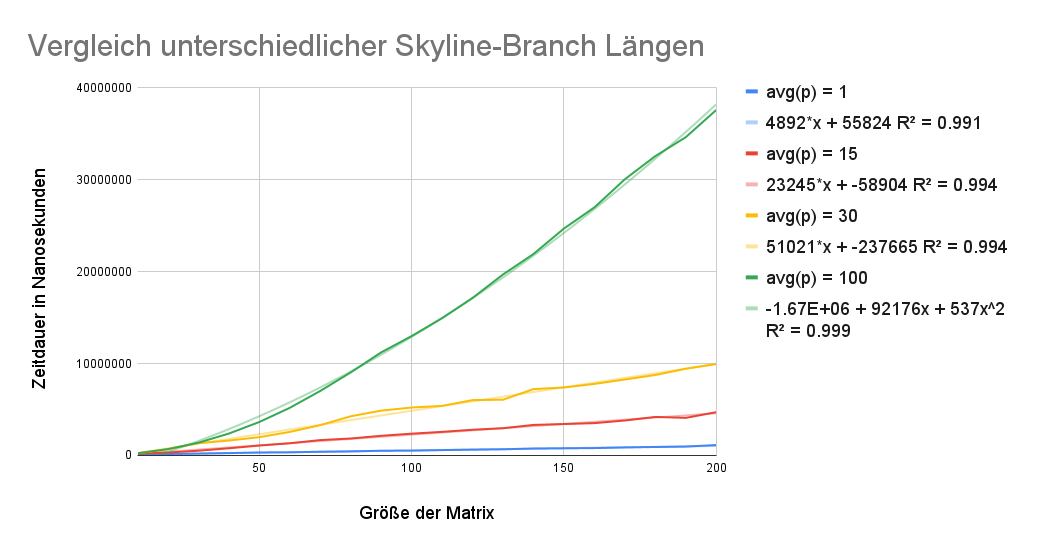
\includegraphics[width=0.9\linewidth]{vergleich_unterschiedlicher_branch_len}
		\caption{Für durchschnittliche $p_l$ Werte bis 30 verhält sich der Aufwand fast linear. Bei großen durchschnittlichen $p_l$ Werten, wie etwa 100 ist der Aufwand bereits polynomial.}
		\label{fig:vergleich_unterschiedlicher_branch_len}
	\end{figure}

	Folgende Grafik vergleicht die Laufzeiten der unterschiedlichen Implementierungen aus Aufgabe 3b.

	\begin{figure}[h!]
		\centering
		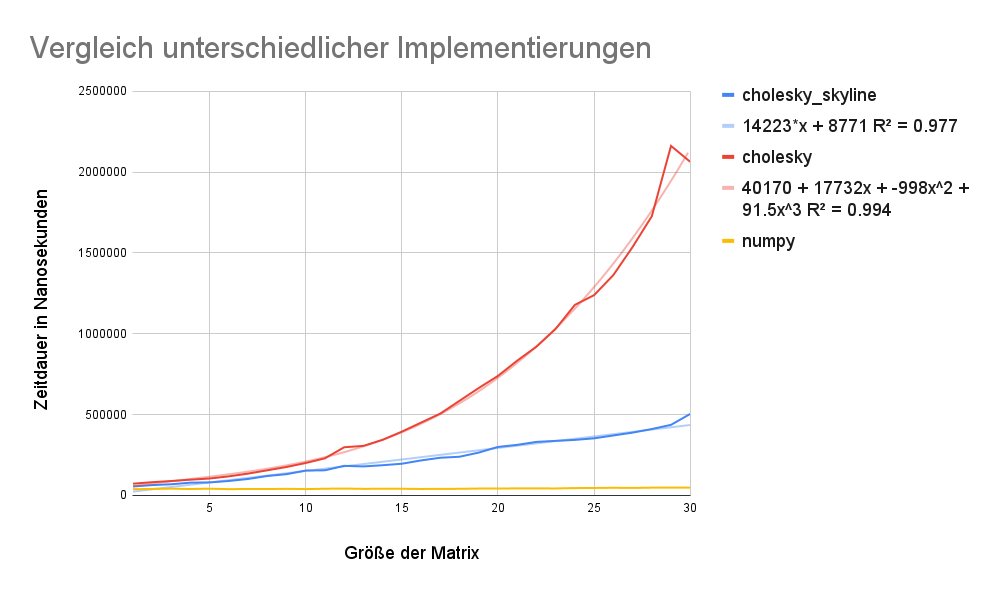
\includegraphics[width=0.9\linewidth]{vergleich_unterschiedlicher_implementierungen}
		\caption{Vergleich des Aufwand der unterschiedlichen Implementierungen für Matrizen bis Größe $30\times 30$ und durchschnittlichem $p_l$ Wert von 10. Der Aufwand von \texttt{cholesky\_skyline} ist deutlich besser, als jener von \texttt{cholesky}, allerdings ist \texttt{numpy.linalg.cholesky}, mit fast konstantem Aufwand, die schnellste Variante.}
		\label{fig:vergleich_unterschiedlicher_implementierungen}
	\end{figure}
	
	Da große Teile von numpy in C geschrieben sind, ist es nicht verwunderlich, dass \texttt{numpy.linalg.cholesky} deutlich schneller läuft als \texttt{choleksy\_skyline}.
\end{ausarbeitung}
\newpage



\appendix
\renewcommand\thesection{Appendix~\Alph{section}:}

\section{Python Implementierung}

\begin{lstlisting}[language=Python, caption=Implementierung der Umwandlung in Skyline-Form sowie der Cholesky Zerlegung für die Skyline-Form]
	import numpy as np
	import matrix_utils
	
	
	class SPDSkylineMatrix:
		values = list()
		
		def __init__(self, matrix):
			if not matrix_utils.is_symmetrical(matrix):
				raise Exception("matrix must be symmetric")
			if not matrix_utils.is_positive_definite(matrix):
				raise Exception("matrix must be positive definite")
			
			for i in range(len(matrix)):
				branch = matrix[:, i][:i + 1].T.tolist()
				branch.reverse()
				while len(branch) > 0 and branch[-1] == 0:
					branch.pop(-1)
				
				self.values.append(branch)
		
		def __getitem__(self, item):
			row_idx, col_idx = item
			row_idx, col_idx = min(row_idx, col_idx), max(row_idx, col_idx)
			
			if row_idx < 0 or col_idx > len(self.values):
				raise Exception("index out of bounds")
			
			col = self.values[col_idx]
			
			if col_idx - row_idx < len(col):
				return col[col_idx - row_idx]
			else:
				return 0
		
		def to_matrix(self):
			matrix = np.zeros((len(self.values), len(self.values)))
			
			for i in range(len(self.values)):
				for j in range(len(self.values[i])):
					matrix[i - j, i] = self.values[i][j]
					matrix[i, i - j] = self.values[i][j]
			
			return matrix
		
		def cholesky(self):
			l = np.zeros((len(self.values), len(self.values)))
			
			max_width = np.max(list(len(lst) for lst in self.values))
			
			for k in range(len(self.values)):
				start_idx = k - len(self.values[k]) + 1
				s = np.dot(l[k][start_idx:k], l[k][start_idx:k])
				l[k, k] = np.sqrt(self[k, k] - s)
				
				for i in range(k + 1, min(k + max_width, len(self.values))):
					if k > i - len(self.values[i]):
						s = np.dot(l[i][start_idx:k], l[k][start_idx:k])
						l[i, k] = (self[i, k] - s) / l[k, k]
			
			return l
\end{lstlisting}

\end{document}
